% Source-authoritative solutions. N(mean,variance); Tri(min,max,mode); Exp(rate).
\makeatletter
\def\input@path{{./}{../}{../../}{../../../}{../../../../}{preamble/}{../preamble/}{../../preamble/}{../../../preamble/}{../../../../preamble/}{book2026-2027/preamble/}}
\makeatother
\input{preamble.tex}
\input{graphs/uniform_linear_probability_distributions.tex}
\input{graphs/G11_C4.tex}
\input{graphs/G11_Histograms.tex}
\usepackage{needspace}
\newgeometry{margin=0.65in,top=0.55in,bottom=0.65in}
\linespread{1.12}
\setlength{\parskip}{5pt}
\setcounter{tocdepth}{1}
\setcounter{secnumdepth}{2}
% Keep the shared scored-section interface; allow long TOC titles to wrap locally.
\renewcommand{\TOCScoredTitle}[2]{\texorpdfstring{#1\quad\sscore{#2}}{#1}}
\newcommand{\SolvedGraph}[2]{\par\smallskip\noindent\begin{minipage}{\linewidth}\centering\textbf{\small #1}\par #2\end{minipage}\par\smallskip}
% Stage numbers reset for each task; hyperlink destinations include the task name.
\newcounter{solutionstage}[section]
\renewcommand{\theHsolutionstage}{\CurrentTask.\arabic{solutionstage}}
\newcommand{\SolutionStage}[2]{\Needspace{5\baselineskip}\refstepcounter{solutionstage}%
\subsubsection*{Stage \arabic{solutionstage}: #2}\label{stage:\CurrentTask:#1}}
\newcommand{\SolutionTask}[2]{\def\CurrentTask{#1}\setcounter{solutionstage}{0}%
\Needspace{6\baselineskip}\phantomsection\label{sol:#1}\subsubsection*{Solution: #2}}
\newcommand{\TaskReturn}[1]{\par\nopagebreak[4]\begingroup\small
\noindent\hyperref[task:#1]{Return to this task}\nopagebreak[4]\secInicio[prob:\CurrentProblem]\endgroup}
% Local diagrams are needed for wraparound and the disjoint exponential tails.
\newcommand{\CycleDiagram}[4]{%
\begin{tikzpicture}[x=0.16cm,y=1cm]
\draw[->] (-1,0)--(51,0) node[right]{min};
\fill[blue!30] (0,0) rectangle (#1,0.6);
\fill[blue!30] (#2,0) rectangle (48,0.6);
\draw (0,0) rectangle (48,0.6);
\draw (0,0)--(0,-0.1) node[below]{$0$};
\draw (#1,0)--(#1,-0.1) node[below=10pt]{$#3$};
\draw (#2,0)--(#2,-0.1) node[below=10pt]{$#4$};
\draw (48,0)--(48,-0.1) node[below]{$48$};
\draw[->,thick] (47,1.0) to[bend right=12] node[above]{restart: $48\equiv0$} (1,1.0);
\end{tikzpicture}}
\newcommand{\NorthDiagram}[2]{%
\begin{tikzpicture}[scale=0.85]
\fill[blue!30] (0,0)--({90-#1}:2) arc[start angle={90-#1},end angle={90+#1},radius=2]--cycle;
\draw[thick] (0,0) circle (2);
\draw[->] (0,0)--(90:2.65) node[above]{North ($0$)};
\draw[dashed] (0,0)--({90-#1}:2.2);
\draw[dashed] (0,0)--({90+#1}:2.2);
\node[anchor=west] at ({90-#1}:2.35){$+#2$};
\node[anchor=east] at ({90+#1}:2.35){$-#2$};
\node at (0,-2.45){Full circle: $360^\circ=2\pi$ rad};
\end{tikzpicture}}

\renewcommand{\ExponentialProbabilityGraph}[3]{%
\begin{center}\begin{tikzpicture}
\begin{axis}[width=11cm,height=4.8cm,axis lines=left,xmin=0,xmax={#3+2},ymin=0,ymax={1.35*#1},xlabel={$t$},ylabel={$f_T(t)$},xtick={0,#2,#3},ytick=\empty,clip=false]
\addplot[domain=#2:#3,samples=100,draw=none,fill=blue!30]{#1*exp(-#1*x)}\closedcycle;
\addplot[domain=0:{#3+2},samples=120,thick]{#1*exp(-#1*x)};
\addplot[dashed] coordinates {(#2,0)(#2,{#1*exp(-#1*#2)})};
\addplot[dashed] coordinates {(#3,0)(#3,{#1*exp(-#1*#3)})};
\node at (axis cs:{(#2+#3)/2},{0.20*#1}) {$P(#2<T<#3)$};
\node[anchor=west] at (axis cs:{0.25*(#2+#3)},{1.12*#1}) {$f_T(t)=#1e^{-#1t}$};
\end{axis}\end{tikzpicture}\end{center}}
\title{Grade 11 -- Term 1\\C1--C7 Catch-up Exam Version 2 Solutions\\\large Continuous distributions and sample data}
\author{Global Economics -- 2026--2027}
\date{}
\hypersetup{pdftitle={Grade 11 Term 1 C1--C7 Catch-up Exam Version 2 Solutions}}
\begin{document}
\maketitle
\phantomsection\label{toc}\tableofcontents
\clearpage
\section*{Learning objective}
Identify probability distributions and their supports; use geometric interval probabilities and exponential waiting times; calculate theoretical moments, empirical probabilities, and sample statistics; and interpret errors relative to theoretical models in economic and operational contexts.\section*{Evaluated criteria}
	\textbf{C1.} Characterises discrete and continuous random variables, identifies suitable distributions and supports, and interprets density and cumulative probability in context.\par
	\textbf{C2.} Applies uniform and triangular models and constant or piecewise-linear densities to interval probabilities using geometric areas.\par
	\textbf{C3.} Uses circular geometry and arc proportions to calculate probabilities for uniform timing and directions around a circle.\par
	\textbf{C4.} Applies exponential models to constant-rate waiting times, infers event rates, and assesses model suitability.\par
	\textbf{C5.} Calculates and interprets the mean, variance, and standard deviation of continuous distributions using standard formulas.\par
	\textbf{C6.} Estimates interval probabilities using sample relative frequencies and compares them with theoretical probabilities.\par
	\textbf{C7.} Calculates sample means, variances, and standard deviations for different sample sizes and data representations and compares them with theory.
\section*{Assessment information}
Each task shows its points. Passing requires \textbf{at least 5 cumulative points per criterion, including previous learning activities}.
Show all procedures; answers without the required procedure receive no credit.
Partial credit may be awarded for a correct method with arithmetic errors.
Missing names or late submissions incur a 1-point deduction per criterion.
\begin{center}
\begin{tabular}{c|rrrrrrr|r}
Criterion&C1&C2&C3&C4&C5&C6&C7&Total\\\hline
Points&6&6&6&7&6&6&6&43
\end{tabular}
\end{center}
\textbf{Conventions.} $N(\mu,\sigma^2)$ uses mean and variance;
$\operatorname{Tri}(a,b,c)$ means minimum, maximum and mode;
$\operatorname{Exp}(\lambda)$ uses the rate parameter.
Supports include their finite boundary points; endpoint inclusion does not affect continuous probabilities.
Probabilities are rounded to four decimal places (percentages to two), statistics, rates and times to three where needed, and percentage errors to two.
All errors use unrounded results. Sample variance uses $n-1$.
Blue task text links to its solution; each solution links back to its task. The arrows return to the problem and contents.


\clearpage\def\CurrentProblem{models}\sectionScored{Models in Colombian operations}{C1-\sml{6}}{prob:models}
\textbf{For each variable below}, classify it as discrete or continuous, identify its distribution, parameters and support, and briefly justify your choice.

\QuestionsTasks[prob:models]{
{1}/{sol:models-a}/{\phantomsection\label{task:models-a}\textbf{1. Municipal compost participation.} A programme records (a) whether a randomly selected household sorts organic waste correctly (1 if correct, 0 otherwise); and (b) the number sorting correctly among 35 households. Households sort correctly independently with probability 0.86. \score{1}},
{1}/{sol:models-b}/{\phantomsection\label{task:models-b}\textbf{2. Water-meter auditing.} A utility records (a) the number of independent tests up to and including the first faulty meter, with constant fault probability 0.06; and (b) a calibration error on $[-2,4]$ litres, with equal probabilities for equal-length intervals and no errors outside this range. Give (a) the probability of the first fault on test $k$ and (b) the density function. \score{1}},
{1}/{sol:models-c}/{\phantomsection\label{task:models-c}\textbf{3. Cultural-centre bookings.} A centre records (a) the number of rehearsal bookings in one hour: arrivals are independent at a constant rate of 3 per hour, one at a time, with negligible multiple arrivals in sufficiently short intervals; and (b) room-reset time on $[8,26]$ minutes: its density rises linearly from zero at 8 to a single peak at 15, then falls linearly to zero at 26, and is zero elsewhere. \score{1}},
{1}/{sol:models-d}/{\phantomsection\label{task:models-d}\textbf{4. Solar-energy monitoring.} A cooperative records (a) the usable battery-bank fraction at sunset on $[0.2,0.9]$: its density rises linearly from zero at 0.2 to its maximum at 0.9 and is zero elsewhere; and (b) sensor error with an exact symmetric bell curve on the real line, centred at 1 watt with standard deviation 3 watts. For (a), find the normalised density function and maximum height. \score{1}},
{1}/{sol:models-e}/{\phantomsection\label{task:models-e}\textbf{5. Agricultural training.} A service records (a) the number of cancellations among 45 independently booked places, each cancelled with probability 0.07; and (b) the number of registration calls over four days: arrivals are independent at a constant rate of 6 per day, one at a time, with negligible multiple arrivals in sufficiently short intervals. \score{1}},
{1}/{sol:models-f}/{\phantomsection\label{task:models-f}\textbf{6. Community-kitchen planning.} A kitchen studies (a) vegetable-batch preparation time from 12 to 36 minutes, with short times most common and density decreasing steadily to zero at the upper limit; and (b) daily rice use, symmetric around 18 kg, with values farther from 18 less common and standard deviation 2.5 kg. For each, discuss whether the distribution and support are uniquely determined. Propose a model, state any additional assumptions, and distinguish model support from possible physical values. Give the density function for (a) under your assumption. \score{1}}
}

\SolutionTask{models-a}{Compost participation}
\textbf{(a)} Discrete: $X\sim\operatorname{Bernoulli}(0.86)$, support $\{0,1\}$. One household gives a single correct/incorrect outcome.
\textbf{(b)} Discrete: $Y\sim\operatorname{Bin}(35,0.86)$, support $\{0,1,\ldots,35\}$. This counts successes in 35 independent trials with the same probability.
\TaskReturn{models-a}

\SolutionTask{models-b}{Water-meter auditing}
\textbf{(a)} Discrete: $X\sim\operatorname{Geom}(0.06)$, support $\{1,2,\ldots\}$. Count every test up to and including the first faulty meter; $P(X=k)=0.94^{k-1}(0.06)$.
\textbf{(b)} Continuous: $Y\sim U(-2,4)$ litres, support $[-2,4]$ L. Equal-length intervals have equal probabilities, so $f(y)=1/(4-(-2))=1/6$ L$^{-1}$ on the support and zero elsewhere.
\TaskReturn{models-b}

\SolutionTask{models-c}{Cultural-centre bookings}
\textbf{(a)} Discrete: $X\sim\operatorname{Poisson}(3)$, support $\{0,1,2,\ldots\}$. The one-hour mean is $3\times1=3$ bookings; the stated conditions define a Poisson process.
\textbf{(b)} Continuous: $Y\sim\operatorname{Tri}(8,26,15)$ minutes, support $[8,26]$ min. The straight branches specify a triangular density with mode 15.
\TaskReturn{models-c}

\SolutionTask{models-d}{Solar-energy monitoring}
\textbf{(a)} Continuous: increasing-linear density, equivalently $X\sim\operatorname{Tri}(0.2,0.9,0.9)$, support $[0.2,0.9]$. Normalisation gives height $2/0.7=20/7$ and $f(x)=2(x-0.2)/(0.7)^2=200(x-0.2)/49$ on this support, zero elsewhere. The fraction is unitless; its mode is 0.9.
\textbf{(b)} Continuous: $Y\sim N(1,9)$ in watts, support $\mathbb R$. The exact symmetric bell curve identifies normality, with SD 3 W and variance $3^2=9$ W$^2$.
\TaskReturn{models-d}

\SolutionTask{models-e}{Agricultural training}
\textbf{(a)} Discrete: $X\sim\operatorname{Bin}(45,0.07)$, support $\{0,1,\ldots,45\}$. These are 45 independent cancellation trials with constant probability.
\textbf{(b)} Discrete: $Y\sim\operatorname{Poisson}(24)$, support $\{0,1,2,\ldots\}$. The four-day mean is $6\times4=24$ calls; 6 is a daily rate, not the four-day count parameter.
\TaskReturn{models-e}

\SolutionTask{models-f}{Community-kitchen planning}
\textbf{(a)} Continuous, support $[12,36]$ min. ``Decreases steadily'' does not uniquely establish a straight-line density. \emph{If a decreasing straight line is intended}, use $X\sim\operatorname{Tri}(12,36,12)$ with $f(x)=(36-x)/288$ on this support and zero elsewhere. Its height is $2/24=1/12$ min$^{-1}$; no extra parameter is needed under this assumption.
\textbf{(b)} Continuous rice use. Symmetric concentration near 18 kg and SD 2.5 kg do not uniquely determine normality or full support. \emph{If normality is assumed}, $Y\sim N(18,6.25)$ in kg, model support $\mathbb R$, with variance $2.5^2=6.25$ kg$^2$. Physical rice use is nonnegative, but its exact physical support is not supplied. These are candidate models under explicit assumptions.
\TaskReturn{models-f}

\clearpage\def\CurrentProblem{stall}\sectionScored{Seedling-tray preparation}{C2-\sml{6}}{prob:stall}
At a Boyac\'a nursery, tray-filling and seeding time $S$ has support $[4,28]$ minutes. Its density rises linearly from zero at 4 to a single maximum at 14, then falls linearly to zero at 28; it is zero elsewhere.

\QuestionsTasks[prob:stall]{
{2}/{sol:stall-a}/{\phantomsection\label{task:stall-a}Identify the model and support, sketch the density, find its maximum height and full piecewise formula (including outside the support), and calculate $P(8\le S\le22)$ using geometric areas. \score{3}},
{2}/{sol:stall-b}/{\phantomsection\label{task:stall-b}Change the support to $[2,34]$ minutes, keeping zero density at both endpoints and linear sides meeting at the mode of 14 minutes. Identify the new model, sketch its density, find its maximum height and full piecewise formula, and recalculate $P(8\le S\le22)$ using geometric areas. \score{3}}
}

\SolutionTask{stall-a}{Original range}

\SolutionStage{1}{Support and shape}
$S\sim\operatorname{Tri}(4,28,14)$ has support $[4,28]$ min. The density rises from $(4,0)$ to $(14,H)$ and falls to $(28,0)$.
\SolvedGraph{Support and triangular shape; horizontal coordinate in minutes}{\CompactDensityCoordinatesGraph{2}{30}{0.11}{4,14,28}{4,14,28}{0,0.08333333333333333}{s}{0,$H$}{(4,0) (14,0.08333333333333333) (28,0)}}
\SolutionStage{2}{Total area = 1}
The triangle area is $\tfrac12\times\text{base}\times\text{height}$, so
\[1=\frac12(28-4)H\quad\Longrightarrow\quad H=\frac2{24}=\frac{1}{12}\ \mathrm{min}^{-1}.\]
\SolutionStage{3}{Complete piecewise pdf}
Use $m=(y_2-y_1)/(x_2-x_1)$ and $q=y_1-mx_1$ in $f(s)=ms+q$.
For the rising line through $(4,0)$ and $(14,\frac{1}{12})$,
\[m_1=\frac{\frac{1}{12}-0}{14-4}=\frac{1}{120},\qquad q_1=0-(\frac{1}{120})(4)=\frac{-1}{30},\qquad f_1(s)=\frac{s-4}{120}.\]
For the falling line through $(14,\frac{1}{12})$ and $(28,0)$,
\[m_2=\frac{0-\frac{1}{12}}{28-14}=\frac{-1}{168},\qquad q_2=0-(\frac{-1}{168})(28)=\frac{1}{6}.\]
Thus the complete density is
\[f(s)=\begin{cases}\dfrac{s-4}{120},&4\le s\le14,\\[1mm]\dfrac{28-s}{168},&14<s\le28,\\[1mm]0,&\text{otherwise}.\end{cases}\]
The branches meet at height $\frac{1}{12}$, are nonnegative, and enclose total area 1.
\Needspace{10cm}\SolutionStage{4}{Probability by complementary tail triangles}
The interval straddles the mode; both tails must be removed:
\[P(8\le S\le22)=1-\frac12(8-4)f(8)-\frac12(28-22)f(22).\]
Here $f(8)=(8-4)/120=\frac{1}{30}$ and $f(22)=(28-22)/168=\frac{1}{28}$ min$^{-1}$.
\[\begin{aligned}P&=1-\tfrac12(4)(\frac{1}{30})-\tfrac12(6)(\frac{1}{28})\\
&=1-\frac{1}{15}-\frac{3}{28}=\boxed{\frac{347}{420}\approx0.8262=82.62\%}.\end{aligned}\]
\SolvedGraph{Shaded event: $8\le S\le22$; $s$ in minutes}{\COneGraph[s]{4}{28}{(x<=14)*((x-4)/120)+(x>14)*((28-x)/168)}{8}{22}{4,8,14,22,28}{0.11}}
Density has units min$^{-1}$. Integrating over $[8,14]$ and $[14,22]$ gives the same probability.
\TaskReturn{stall-a}

\SolutionTask{stall-b}{Changed range}
\textbf{What stays fixed.} The mode is 14 min, the event is $[8,22]$, and both branches remain straight. Only the support endpoints change.\par
\SolutionStage{1}{Support and shape}
$S\sim\operatorname{Tri}(2,34,14)$ has support $[2,34]$ min. The density rises from $(2,0)$ to $(14,H)$ and falls to $(34,0)$.
\SolvedGraph{Support and triangular shape; horizontal coordinate in minutes}{\CompactDensityCoordinatesGraph{0}{36}{0.11}{2,14,34}{2,14,34}{0,0.0625}{s}{0,$H$}{(2,0) (14,0.0625) (34,0)}}
\SolutionStage{2}{Total area = 1}
The triangle area is $\tfrac12\times\text{base}\times\text{height}$, so
\[1=\frac12(34-2)H\quad\Longrightarrow\quad H=\frac2{32}=\frac{1}{16}\ \mathrm{min}^{-1}.\]
\SolutionStage{3}{Complete piecewise pdf}
Use $m=(y_2-y_1)/(x_2-x_1)$ and $q=y_1-mx_1$ in $f(s)=ms+q$.
For the rising line through $(2,0)$ and $(14,\frac{1}{16})$,
\[m_1=\frac{\frac{1}{16}-0}{14-2}=\frac{1}{192},\qquad q_1=0-(\frac{1}{192})(2)=\frac{-1}{96},\qquad f_1(s)=\frac{s-2}{192}.\]
For the falling line through $(14,\frac{1}{16})$ and $(34,0)$,
\[m_2=\frac{0-\frac{1}{16}}{34-14}=\frac{-1}{320},\qquad q_2=0-(\frac{-1}{320})(34)=\frac{17}{160}.\]
Thus the complete density is
\[f(s)=\begin{cases}\dfrac{s-2}{192},&2\le s\le14,\\[1mm]\dfrac{34-s}{320},&14<s\le34,\\[1mm]0,&\text{otherwise}.\end{cases}\]
The branches meet at height $\frac{1}{16}$, are nonnegative, and enclose total area 1.
\Needspace{10cm}\SolutionStage{4}{Probability by complementary tail triangles}
The interval straddles the mode; both tails must be removed:
\[P(8\le S\le22)=1-\frac12(8-2)f(8)-\frac12(34-22)f(22).\]
Here $f(8)=(8-2)/192=\frac{1}{32}$ and $f(22)=(34-22)/320=\frac{3}{80}$ min$^{-1}$.
\[\begin{aligned}P&=1-\tfrac12(6)(\frac{1}{32})-\tfrac12(12)(\frac{3}{80})\\
&=1-\frac{3}{32}-\frac{9}{40}=\boxed{\frac{109}{160}\approx0.6813=68.13\%}.\end{aligned}\]
\SolvedGraph{Shaded event: $8\le S\le22$; $s$ in minutes}{\COneGraph[s]{2}{34}{(x<=14)*((x-2)/192)+(x>14)*((34-x)/320)}{8}{22}{2,8,14,22,34}{0.11}}
Density has units min$^{-1}$. Integrating over $[8,14]$ and $[14,22]$ gives the same probability.
\TaskReturn{stall-b}

\clearpage\def\CurrentProblem{cycle}\sectionScored{A repeating irrigation cycle}{C3-\sml{3}}{prob:cycle}
A flower farm's pressure fluctuation occurs uniformly within a repeating 48-minute irrigation cycle, starting at minute 0 and restarting immediately after minute 48.

\QuestionsTasks[prob:cycle]{
{3}/{sol:cycle-a}/{\phantomsection\label{task:cycle-a}Find the probability of a fluctuation from minute 41 through the restart to minute 9 of the next cycle. State the event as interval(s) within one cycle. \score{1}},
{3}/{sol:cycle-b}/{\phantomsection\label{task:cycle-b}Find the probability of a fluctuation within 150 seconds on either side of the cycle start. State the event as interval(s) within one cycle. \score{2}}
}

\SolutionTask{cycle-a}{Window through the restart}
Let $U\sim U(0,48)$ represent position in minutes, with density $1/48$ min$^{-1}$ on $[0,48)$.
The window splits into $[41,48)$ and $[0,9]$, of lengths 7 and 9 minutes.
\SolvedGraph{The shaded lengths meet through the restart}{\CycleDiagram{9}{41}{9}{41}}
\[P=\frac{(48-41)+(9-0)}{48}=\boxed{\frac13\approx0.3333=33.33\%}.\]
\TaskReturn{cycle-a}

\SolutionTask{cycle-b}{Tolerance on both sides}
Convert first: $150\ \mathrm s=150/60=5/2$ min on \emph{each} side.
The intervals are $[0,5/2]$ and $[48-5/2,48)=[91/2,48)$.
\SolvedGraph{Two equal pieces beside the cycle start}{\CycleDiagram{2.5}{45.5}{5/2}{91/2}}
\[P=\frac{5/2+5/2}{48}=\boxed{\frac5{48}\approx0.1042=10.42\%}.\]
Endpoints have probability zero; their inclusion does not change either answer.
\TaskReturn{cycle-b}

\clearpage\def\CurrentProblem{drone}\sectionScored{Direction of a floating current marker}{C3-\sml{3}}{prob:drone}
A river-monitoring team's floating marker has an initial direction uniform around a full circle. A bank marker indicates north. Angular tolerances apply on \textbf{both sides} of north, including wraparound.

\QuestionsTasks[prob:drone]{
{3}/{sol:drone-a}/{\phantomsection\label{task:drone-a}For each tolerance ($\pi/8$ radians and $18^\circ$ from north), state the event as angular intervals with north at zero and calculate its probability. Identify the larger probability, give the difference in percentage points, and calculate the relative increase from the $18^\circ$ probability. \score{3}}
}

\SolutionTask{drone-a}{Angular probabilities and comparison}
Uniform directions give probability equal to favourable angle divided by full-circle angle. Count \emph{both sides} of north.
\SolvedGraph{Two wraparound sectors centred at north}{\NorthDiagram{22.5}{\pi/8}\hspace{1.4cm}\NorthDiagram{18}{18^\circ}}
In radians, the event is $[0,\pi/8]\cup[2\pi-\pi/8,2\pi)$:
\[P_{\pi/8}=\frac{2(\pi/8)}{2\pi}=\boxed{\frac18=0.1250=12.50\%}.\]
In degrees, the event is $[0,18]\cup[342,360)$:
\[P_{18^\circ}=\frac{2(18^\circ)}{360^\circ}=\boxed{\frac1{10}=0.1000=10.00\%}.\]
The $\pi/8$ tolerance (22.5 degrees on each side) gives greater probability:
\[\Delta P=\frac18-\frac1{10}=\boxed{\frac1{40}=0.0250},\]
an absolute difference of \textbf{2.50 percentage points}.
Using the 18-degree probability as baseline, the relative increase is
\[100\frac{1/40}{1/10}\%=25.00\%.\]
\TaskReturn{drone-a}

\clearpage\def\CurrentProblem{charging}\sectionScored{Public-library return arrivals}{C4-\sml{3}}{prob:charging}
Returns enter a public library's automated chute as a Poisson process, with a different constant rate in each scenario below. Let $T$ be the waiting time in minutes from a fixed observation time to the next return.

For each scenario, identify the waiting-time model, rate in returns per minute and support, and calculate the probability. Give the general density function and briefly justify the model.

\QuestionsTasks[prob:charging]{
{4}/{sol:charging-a}/{\phantomsection\label{task:charging-a}With an average of 7 returns every 35 minutes, find $P(T<3)$. \score{0.5}},
{4}/{sol:charging-b}/{\phantomsection\label{task:charging-b}With a mean waiting time of 5 minutes between returns, find $P(T>8)$. \score{0.5}},
{4}/{sol:charging-c}/{\phantomsection\label{task:charging-c}With an average of 4 returns every 25 minutes, find $P(1<T<6)$. \score{1}},
{4}/{sol:charging-d}/{\phantomsection\label{task:charging-d}With an average of 18 returns per hour, find $P(T<2\text{ or }T>7)$. \score{1}}
}

\Needspace{8cm}

\SolutionTask{charging-a}{Less than three minutes}
The rate is $\lambda_1=7/35=1/5=0.200$ returns/min.
For $T\sim\operatorname{Exp}(\lambda_1)$, $P(T<t)=1-e^{-\lambda_1t}$.
\[P(T<3)=1-e^{-(1/5)(3)}=\boxed{1-e^{-3/5}\approx0.4512=45.12\%}.\]
\SolvedGraph{Shaded event; $t$ in minutes and $f_T(t)$ in inverse minutes}{\ExponentialLessThanGraph{0.2}{3}{6}}
\TaskReturn{charging-a}

\Needspace{8cm}

\SolutionTask{charging-b}{More than eight minutes}
A mean wait of 5 min gives $\lambda_2=1/E(T)=1/5=0.200$ returns/min.
Use the survival formula $P(T>t)=e^{-\lambda_2t}$.
\[P(T>8)=e^{-(1/5)(8)}=\boxed{e^{-8/5}\approx0.2019=20.19\%}.\]
\SolvedGraph{Shaded event; $t$ in minutes and $f_T(t)$ in inverse minutes}{\ExponentialGreaterThanGraph{0.2}{8}{5}}
The shaded right tail continues beyond the plotted edge to infinity.
\TaskReturn{charging-b}

\Needspace{8cm}

\SolutionTask{charging-c}{Between one and six minutes}
The separate rate is $\lambda_3=4/25=0.160$ returns/min.
For an interval, $P(a<T<b)=e^{-\lambda_3a}-e^{-\lambda_3b}$.
\[P(1<T<6)=e^{-(4/25)(1)}-e^{-(4/25)(6)}=\boxed{e^{-4/25}-e^{-24/25}\approx0.4693=46.93\%}.\]
\SolvedGraph{Shaded event; $t$ in minutes and $f_T(t)$ in inverse minutes}{\ExponentialProbabilityGraph{0.16}{1}{6}}
\TaskReturn{charging-c}

\Needspace{8cm}

\SolutionTask{charging-d}{Outside two to seven minutes}
Convert the hourly rate: $\lambda_4=18/60=3/10=0.300$ returns/min.
The two tails are disjoint, so $P(T<a\text{ or }T>b)=(1-e^{-\lambda_4a})+e^{-\lambda_4b}$.
\[P(T<2\text{ or }T>7)=1-e^{-(3/10)(2)}+e^{-(3/10)(7)}=\boxed{1-e^{-3/5}+e^{-21/10}\approx0.5736=57.36\%}.\]
\SolvedGraph{Both shaded tails; right tail continues to infinity}{
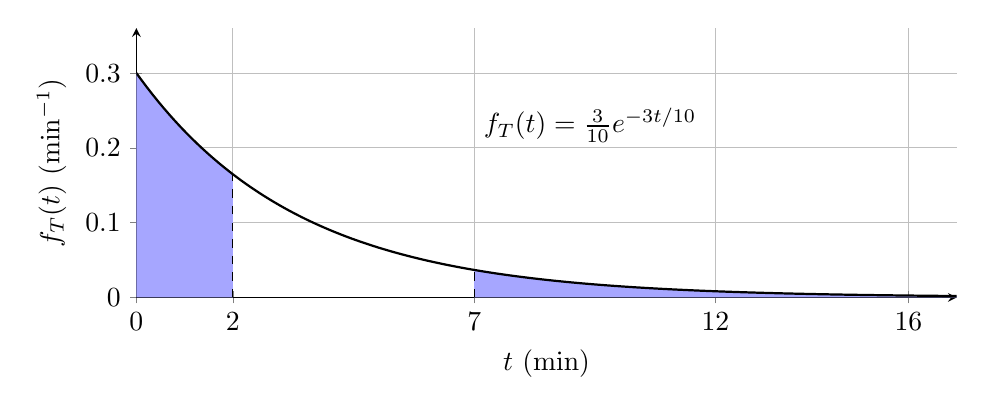
\begin{tikzpicture}\begin{axis}[width=12cm,height=5cm,axis lines=left,xmin=0,xmax=17,ymin=0,ymax=0.36,xlabel={$t$ (min)},ylabel={$f_T(t)$ (min$^{-1}$)},xtick={0,2,7,12,16},grid=major]
\addplot[domain=0:2,samples=60,draw=none,fill=blue!35]{0.3*exp(-0.3*x)}\closedcycle;
\addplot[domain=7:17,samples=100,draw=none,fill=blue!35]{0.3*exp(-0.3*x)}\closedcycle;
\addplot[domain=0:17,samples=150,thick]{0.3*exp(-0.3*x)};
\addplot[dashed] coordinates {(2,0)(2,0.16464349)};
\addplot[dashed] coordinates {(7,0)(7,0.03673693)};
\node[anchor=west] at (axis cs:7,0.23){$f_T(t)=\frac3{10}e^{-3t/10}$};
\end{axis}\end{tikzpicture}}
For all four scenarios, $f_T(t)=\lambda e^{-\lambda t}$ for $t\ge0$, zero otherwise, with support $[0,\infty)$. The constant-rate Poisson assumption makes exponential waiting times appropriate.
\TaskReturn{charging-d}

\Needspace{14\baselineskip}\def\CurrentProblem{receipts}\sectionScored{Bicycle-hire arrival rates}{C4-\sml{2}}{prob:receipts}
At a municipal bicycle-hire kiosk, rentals start as a Poisson process with different constant morning and afternoon rates. Let $T_m,T_a$ be the respective waiting times in minutes from a fixed time in each shift to the next rental. Assume each shift continues throughout the wait.

\QuestionsTasks[prob:receipts]{
{4}/{sol:receipts-a}/{\phantomsection\label{task:receipts-a}In the morning, $P(T_m>12)=0.35$. Infer the rate in rental starts per minute and per hour. \score{1}},
{4}/{sol:receipts-b}/{\phantomsection\label{task:receipts-b}In the afternoon, $P(T_a<9)=0.72$. Infer the rate in rental starts per minute and per hour. \score{1}}
}

\SolutionTask{receipts-a}{Morning rate from survival}
Use $P(T_m>t)=e^{-\lambda_m t}$:
\[0.35=e^{-12\lambda_m}\ \Longrightarrow\ \ln(0.35)=-12\lambda_m\ \Longrightarrow\ \lambda_m=-\frac{\ln(0.35)}{12}\approx0.087\ \text{starts/min}.\]
Convert the exact rate to hourly units:
\[60\lambda_m=-5\ln(0.35)\approx\boxed{5.249\ \text{starts/hour}}.\]
\TaskReturn{receipts-a}

\SolutionTask{receipts-b}{Afternoon rate from a cumulative probability}
Use $P(T_a<t)=1-e^{-\lambda_a t}$:
\[0.72=1-e^{-9\lambda_a}\ \Longrightarrow\ e^{-9\lambda_a}=0.28\ \Longrightarrow\ -9\lambda_a=\ln(0.28).\]
\[\lambda_a=-\frac{\ln(0.28)}9\approx0.141\ \text{starts/min},\qquad60\lambda_a=-\frac{20}3\ln(0.28)\approx\boxed{8.486\ \text{starts/hour}}.\]
\TaskReturn{receipts-b}

\Needspace{14\baselineskip}\def\CurrentProblem{payments}\sectionScored{Two recycling collection gates}{C4-\sml{2}}{prob:payments}
Vehicle entries at recycling gates A and B follow independent constant-rate Poisson processes. From a fixed observation time, A's next entry has probability 0.84 of occurring within 4 minutes; B's has probability 0.60 of taking more than 4 minutes. Count both gates' entries from this same time.

\QuestionsTasks[prob:payments]{
{4}/{sol:payments-a}/{\phantomsection\label{task:payments-a}Infer both rates in entries per minute and state the expected-count functions. Find when A\textquotesingle s expected count exceeds B\textquotesingle s by 4, in minutes, and explain what this time means for actual entries. \score{2}}
}

\SolutionTask{payments-a}{Rates and expected-count difference}
For A the given probability is cumulative:
\[0.84=1-e^{-4\lambda_A}\ \Longrightarrow\ e^{-4\lambda_A}=0.16\ \Longrightarrow\ \lambda_A=-\frac{\ln(0.16)}4\approx0.458\ \text{entries/min}.\]
For B it is a survival probability:
\[0.60=e^{-4\lambda_B}\ \Longrightarrow\ \lambda_B=-\frac{\ln(0.60)}4\approx0.128\ \text{entries/min}.\]
Define $N_A(t),N_B(t)$ as entry counts since the common observation time. For constant-rate Poisson processes,
\[E[N_A(t)]=\lambda_A t,\qquad E[N_B(t)]=\lambda_B t.\]
Thus $E[N_A(t)]-E[N_B(t)]=(\lambda_A-\lambda_B)t$. Since $\lambda_A>\lambda_B$, the required time is positive and finite:
\[t=\frac4{\lambda_A-\lambda_B}=\frac{16}{\ln(0.60/0.16)}=\boxed{\frac{16}{\ln(15/4)}\approx12.105\ \text{min}}.\]
This specifies a difference of 4 in \emph{expected} counts; the actual random count difference need not be 4 at this time.
\TaskReturn{payments-a}

\Needspace{14\baselineskip}\def\CurrentProblem{labelling}\sectionScored{Two document-digitisation desks}{C5-\sml{2}}{prob:labelling}
At a municipal archive, $A$ and $B$ are file-digitisation times in minutes at two desks, both with support $[2,17]$. A's density rises linearly from zero at 2 to its maximum at 17. B has equal probabilities for equal-length intervals within the support. Both densities are zero elsewhere.

\QuestionsTasks[prob:labelling]{
{5}/{sol:labelling-a}/{\phantomsection\label{task:labelling-a}Identify A\textquotesingle s distribution, parameters and support, and calculate its mean, variance and standard deviation. Interpret the mean in context. \score{1}},
{5}/{sol:labelling-b}/{\phantomsection\label{task:labelling-b}Identify B\textquotesingle s distribution, parameters and support, and calculate its mean, variance and standard deviation. Interpret the mean and standard deviation in context. \score{1}}
}

\SolutionTask{labelling-a}{Increasing-linear digitisation time}
The increasing straight density is an endpoint triangular model: $A\sim\operatorname{Tri}(2,17,17)$, support $[2,17]$ min.
For increasing-linear density on $[a,b]$,
\[\mu=\frac{a+2b}3,\qquad\sigma^2=\frac{(b-a)^2}{18},\qquad\sigma=\sqrt{\sigma^2}.\]
\[E(A)=\frac{2+2(17)}3=12\ \text{min},\qquad\operatorname{Var}(A)=\frac{(17-2)^2}{18}=\frac{25}2=12.500\ \text{min}^2,\]
\[\sigma_A=\sqrt{25/2}\approx3.536\ \text{min}.\]
Over many files, desk A averages 12 minutes per file.
\TaskReturn{labelling-a}

\SolutionTask{labelling-b}{Uniform digitisation time}
Equal-length intervals have equal probabilities, so $B\sim U(2,17)$, support $[2,17]$ min.
The formulas are $\mu=(a+b)/2$, $\sigma^2=(b-a)^2/12$, $\sigma=\sqrt{\sigma^2}$.
\[E(B)=\frac{2+17}2=9.500\ \text{min},\qquad\operatorname{Var}(B)=\frac{(17-2)^2}{12}=\frac{75}4=18.750\ \text{min}^2,\]
\[\sigma_B=\sqrt{75/4}\approx4.330\ \text{min}.\]
Desk B averages 9.5 minutes per file; its time SD is about 4.330 minutes.
\TaskReturn{labelling-b}

\Needspace{14\baselineskip}\def\CurrentProblem{revenue}\sectionScored{Pump maintenance and daily operating costs}{C5-\sml{2}}{prob:revenue}
A rural water association's pump maintenance duration $D$ has support $[2,14]$ hours. Its density falls linearly from its maximum at 2 to zero at 14 and is zero elsewhere.

Daily operating cost $R$, in \textbf{thousands of Colombian pesos (COP)}, has an exact symmetric bell-shaped density on the real line, centred at 2400 with inflection points 2250 and 2550.

\QuestionsTasks[prob:revenue]{
{5}/{sol:revenue-a}/{\phantomsection\label{task:revenue-a}Identify D\textquotesingle s distribution, parameters and support, and calculate its mean, variance and standard deviation. Interpret the mean in context. \score{1}},
{5}/{sol:revenue-b}/{\phantomsection\label{task:revenue-b}Identify R\textquotesingle s distribution and infer its parameters and support. Calculate mean and SD in \textbf{COP} and variance in \textbf{COP$^2$}. Interpret the mean. \score{1}}
}

\SolutionTask{revenue-a}{Decreasing-linear maintenance duration}
The decreasing straight density gives $D\sim\operatorname{Tri}(2,14,2)$, support $[2,14]$ h.
Use $\mu=(2a+b)/3$, $\sigma^2=(b-a)^2/18$, $\sigma=\sqrt{\sigma^2}$:
\[E(D)=\frac{2(2)+14}3=6\ \text{h},\qquad\operatorname{Var}(D)=\frac{(14-2)^2}{18}=8\ \text{h}^2,\qquad\sigma_D=\sqrt8\approx2.828\ \text{h}.\]
The model predicts a long-run average maintenance duration of 6 hours.
\TaskReturn{revenue-a}

\SolutionTask{revenue-b}{Normal cost and conversion to COP}
The exact symmetric bell curve identifies a normal distribution. In thousands of COP, the centre is $\mu_R=2400$.
Normal inflection points are $\mu_R\pm\sigma_R$, so
\[\sigma_R=2550-2400=2400-2250=150,\qquad R\sim N(2400,150^2)=N(2400,22500).\]
Its mathematical support is $\mathbb R$. In these units, mean is $\mu_R$, variance is $\sigma_R^2$, and SD is $\sigma_R$.
Let $Y=1000R$ be cost in COP. The conversion laws are
\[E(cR)=cE(R),\quad\operatorname{Var}(cR)=c^2\operatorname{Var}(R),\quad\operatorname{SD}(cR)=|c|\operatorname{SD}(R).\]
Therefore
\[E(Y)=1000(2400)=2{,}400{,}000\ \text{COP},\]
\[\operatorname{Var}(Y)=1000^2(22500)=22{,}500{,}000{,}000\ \text{COP}^2,\qquad\operatorname{SD}(Y)=1000(150)=150{,}000\ \text{COP}.\]
The association's long-run average daily operating cost is 2,400,000 COP; individual days vary around it.
\TaskReturn{revenue-b}

\Needspace{14\baselineskip}\def\CurrentProblem{repairs}\sectionScored{Museum admissions and audio-guide sessions}{C5-\sml{2}}{prob:repairs}
Museum admissions follow a constant-rate Poisson process averaging 15 per hour. Let $T$ be the interarrival time in minutes.

Audio-guide session duration $S$ has support $[6,27]$ minutes. Its density rises linearly from zero at 6 to a single peak at 15, then falls linearly to zero at 27; it is zero elsewhere.

\QuestionsTasks[prob:repairs]{
{5}/{sol:repairs-a}/{\phantomsection\label{task:repairs-a}Identify T\textquotesingle s distribution, parameters and support, and calculate its mean and SD in minutes and its variance in minutes$^2$. Interpret the mean in context. \score{1}},
{5}/{sol:repairs-b}/{\phantomsection\label{task:repairs-b}Identify S\textquotesingle s distribution, parameters and support, and calculate its mean and SD in minutes and its variance in minutes$^2$. Interpret the mean and standard deviation in context. \score{1}}
}

\SolutionTask{repairs-a}{Exponential interarrival time}
The constant-rate Poisson process gives $T\sim\operatorname{Exp}(\lambda)$, support $[0,\infty)$ min, with $\lambda=15/60=1/4=0.250$ admissions/min.
Use $\mu=1/\lambda$, $\sigma^2=1/\lambda^2$, $\sigma=1/\lambda$:
\[E(T)=\frac1{1/4}=4\ \text{min},\qquad\operatorname{Var}(T)=\frac1{(1/4)^2}=16\ \text{min}^2,\qquad\sigma_T=4\ \text{min}.\]
The mean gap between admissions is 4 minutes.
\TaskReturn{repairs-a}

\SolutionTask{repairs-b}{Triangular audio-guide duration}
The straight branches give $S\sim\operatorname{Tri}(6,27,15)$, support $[6,27]$ min.
For minimum $a$, maximum $b$, mode $c$,
\[\mu=\frac{a+b+c}3,\quad\sigma^2=\frac{a^2+b^2+c^2-ab-ac-bc}{18},\quad\sigma=\sqrt{\sigma^2}.\]
\[E(S)=\frac{6+27+15}3=16\ \text{min}.\]
\[\begin{aligned}\operatorname{Var}(S)&=\frac{6^2+27^2+15^2-6(27)-6(15)-27(15)}{18}\\&=\frac{333}{18}=\frac{37}2=18.500\ \text{min}^2,\end{aligned}\]
\[\sigma_S=\sqrt{37/2}\approx4.301\ \text{min}.\]
The model predicts a mean session of 16 minutes with SD about 4.301 minutes.
\TaskReturn{repairs-b}

\Needspace{14\baselineskip}\def\CurrentProblem{parcels}\sectionScored{Commercial-kitchen water use}{C6-\sml{2}}{prob:parcels}
A catering kitchen records water use $X$ in litres for 50 cleaning batches in two non-overlapping parts. The first 20 observations are:
\[\begin{array}{rrrrr}4.1&4.5&5.0&5.3&5.8\\6.0&6.2&6.7&7.0&7.4\\4.8&5.0&5.5&5.9&6.4\\6.8&7.0&7.2&7.6&8.0\end{array}\]
The remaining 30 observations have this discrete frequency table:
\[\begin{array}{c|rrrrrr}x_i&5.0&5.4&5.8&6.3&7.0&7.5\\\hline f_i&4&6&5&7&3&5\end{array}\]
Combine both parts as one sample. The model gives $P(5\le X<7)=0.58$.

\QuestionsTasks[prob:parcels]{
{6}/{sol:parcels-a}/{\phantomsection\label{task:parcels-a}State the sample size and event count, then calculate the empirical probability. \score{1}},
{6}/{sol:parcels-b}/{\phantomsection\label{task:parcels-b}Calculate its absolute and percentage errors. \score{1}}
}

\SolutionTask{parcels-a}{Empirical probability}
Eligible raw observations are $5.0,5.3,5.8,6.0,6.2,6.7,5.0,5.5,5.9,6.4,6.8$, giving \textbf{11} batches.
Table values $5.0,5.4,5.8,6.3$ contribute $4+6+5+7=22$ batches. Include every 5 and exclude every 7.
The records do not overlap, so $n=20+30=50$ and $k=11+22=33$.
\[\widehat P(5\le X<7)=\frac{33}{50}=0.6600=66.00\%.\]
\TaskReturn{parcels-a}

\SolutionTask{parcels-b}{Absolute and percentage errors}
Use $E=|\widehat P-P_0|$ and $E\%=100E/|P_0|$, using the exact relative frequency:
\[E=\left|\frac{33}{50}-0.58\right|=\frac{2}{25}\approx0.0800.\]
\[E\%=100\frac{\frac{2}{25}}{0.58}\%\approx13.79\%.\]
Probabilities and their errors are unitless.
\TaskReturn{parcels-b}

\Needspace{14\baselineskip}\def\CurrentProblem{transfers}\sectionScored{Produce cooling, grouped data}{C6-\sml{2}}{prob:transfers}
Produce-crate cooling times $X$ in minutes at a packing centre are grouped below. Classes include the left endpoint and exclude the right.
\[\begin{array}{c|rrrr}\text{Class}&[2,7)&[7,12)&[12,17)&[17,22)\\\hline f_i&4&7&6&4\end{array}\]
The model gives $P(7\le X<17)=0.68$.

\QuestionsTasks[prob:transfers]{
{6}/{sol:transfers-a}/{\phantomsection\label{task:transfers-a}State the sample size and event count, then calculate the empirical probability. \score{1}},
{6}/{sol:transfers-b}/{\phantomsection\label{task:transfers-b}Calculate its absolute and percentage errors. \score{1}}
}

\SolutionTask{transfers-a}{Empirical probability}
The complete included classes are $[7,12)$ and $[12,17)$.
Thus $n=4+7+6+4=21$ and $k=7+6=13$. These counts are exact because event endpoints are class boundaries; no midpoint approximation is needed.
\[\widehat P(7\le X<17)=\frac{13}{21}\approx0.6190=61.90\%.\]
\TaskReturn{transfers-a}

\SolutionTask{transfers-b}{Absolute and percentage errors}
Use $E=|\widehat P-P_0|$ and $E\%=100E/|P_0|$, using the exact relative frequency:
\[E=\left|\frac{13}{21}-0.68\right|=\frac{32}{525}\approx0.0610.\]
\[E\%=100\frac{\frac{32}{525}}{0.68}\%\approx8.96\%.\]
Probabilities and their errors are unitless.
\TaskReturn{transfers-b}

\Needspace{14\baselineskip}\def\CurrentProblem{queues}\sectionScored{Battery-swap service, histogram}{C6-\sml{2}}{prob:queues}
The histogram is the only sample record of battery-swap times $X$ at an electric-motorcycle station. The horizontal axis shows minutes; bar heights are frequencies. Equal-width classes include the left endpoint and exclude the right.
\HistogramGraph{(1,4),(4,7),(7,10),(10,13)}{3,9,7,6}{0.94\linewidth}{4.4cm}{blue!25}{3}{1}
The model gives $P(4\le X<10)=0.60$.

\QuestionsTasks[prob:queues]{
{6}/{sol:queues-a}/{\phantomsection\label{task:queues-a}State the sample size and event count, then calculate the empirical probability. \score{1}},
{6}/{sol:queues-b}/{\phantomsection\label{task:queues-b}Calculate its absolute and percentage errors. \score{1}}
}

\SolutionTask{queues-a}{Empirical probability}
Read the four histogram heights as frequencies $3,9,7,6$.
The included complete classes are $[4,7)$ and $[7,10)$, giving $n=3+9+7+6=25$ and $k=9+7=16$. No midpoint approximation is needed.
\[\widehat P(4\le X<10)=\frac{16}{25}=0.6400=64.00\%.\]
\TaskReturn{queues-a}

\SolutionTask{queues-b}{Absolute and percentage errors}
Use $E=|\widehat P-P_0|$ and $E\%=100E/|P_0|$, using the exact relative frequency:
\[E=\left|\frac{16}{25}-0.60\right|=\frac{1}{25}\approx0.0400.\]
\[E\%=100\frac{\frac{1}{25}}{0.60}\%\approx6.67\%.\]
Probabilities and their errors are unitless.
\TaskReturn{queues-b}

\Needspace{14\baselineskip}\def\CurrentProblem{cold-room}\sectionScored{Daily paper use, mixed data}{C7-\sml{2}}{prob:cold-room}
A legal-aid office records paper use in hundreds of sheets on 13 days in two non-overlapping parts: the first five observations are $13,16,18,21,23$; the remaining eight are summarised below:
\[\begin{array}{c|rrr}x_i&13&18&23\\\hline f_i&1&4&3\end{array}\]
Combine both parts as one sample. The theoretical mean is 18 hundreds of sheets and variance is 16 (hundreds of sheets)$^2$.

\QuestionsTasks[prob:cold-room]{
{7}/{sol:cold-room-a}/{\phantomsection\label{task:cold-room-a}State the sample size; calculate the sample mean, variance and standard deviation. Show your frequency summary and weighted sum of squared deviations. \score{1}},
{7}/{sol:cold-room-b}/{\phantomsection\label{task:cold-room-b}Calculate absolute and percentage errors for mean and variance. \score{1}}
}

\SolutionTask{cold-room-a}{Sample statistics from combined data}
The five raw observations contribute one each at $13,16,18,21,23$; the table adds $1,4,3$ at $13,18,23$. The combined actual-value frequencies below require no midpoint estimation.\[\begin{array}{c|rrrrr}x_i&13&16&18&21&23\\\hline f_i&2&1&5&1&4\end{array}\]
Use sample variance with denominator $n-1$:
\[n=\sum f_i=13,\qquad\bar x=\frac{\sum f_ix_i}{n}.\]
\[\bar x=\frac{2(13)+1(16)+5(18)+1(21)+4(23)}{13}=\frac{245}{13}\approx18.846\ \text{hundreds of sheets}.\]
The weighted squared-deviation sum is
\[\begin{aligned}Q&=\sum_i f_i(x_i-\bar x)^2\\&=2\left(13-\frac{245}{13}\right)^2+1\left(16-\frac{245}{13}\right)^2+5\left(18-\frac{245}{13}\right)^2\\&\quad+1\left(21-\frac{245}{13}\right)^2+4\left(23-\frac{245}{13}\right)^2\\&=\frac{1998}{13}\ (\text{hundreds of sheets})^2.\end{aligned}\]
\begin{samepage}
\[s^2=\frac{\sum_i f_i(x_i-\bar x)^2}{n-1}=\frac{\frac{1998}{13}}{13-1}=\frac{333}{26}\approx12.808\ (\text{hundreds of sheets})^2,\]
\[s=\sqrt{s^2}\approx\sqrt{\frac{333}{26}}\approx3.579\ \text{hundreds of sheets}.\]
\end{samepage}
\TaskReturn{cold-room-a}

\SolutionTask{cold-room-b}{Mean and variance errors}
For a statistic $z$ and theoretical value $z_0$, use $E=|z-z_0|$, $E\%=100E/|z_0|$.
Using unrounded statistics:
\[E_{\bar x}=\left|\frac{245}{13}-18\right|=\frac{11}{13}\approx0.846\ \text{hundreds of sheets},\qquad E_{\bar x}\%=100\frac{\frac{11}{13}}{18}\%\approx4.70\%.\]
\[E_{s^2}=\left|\frac{333}{26}-16\right|=\frac{83}{26}\approx3.192\ (\text{hundreds of sheets})^2,\qquad E_{s^2}\%=100\frac{\frac{83}{26}}{16}\%\approx19.95\%.\]
The requested errors concern the mean and variance only.
\TaskReturn{cold-room-b}

\Needspace{14\baselineskip}\def\CurrentProblem{routes}\sectionScored{Compost maturation checks, grouped data}{C7-\sml{2}}{prob:routes}
An urban garden groups times between compost checks in days. Classes include the left endpoint and exclude the right. The theoretical mean is 15 days and variance is 24 days$^2$.
\[\begin{array}{c|rrr}\text{Class}&[5,11)&[11,17)&[17,23)\\\hline f_i&3&2&2\end{array}\]

\QuestionsTasks[prob:routes]{
{7}/{sol:routes-a}/{\phantomsection\label{task:routes-a}State the sample size; calculate the sample mean, variance and standard deviation. Show your frequency summary and weighted sum of squared deviations. \score{1}},
{7}/{sol:routes-b}/{\phantomsection\label{task:routes-b}Calculate absolute and percentage errors for mean and variance. \score{1}}
}

\Needspace{13cm}

\SolutionTask{routes-a}{Sample statistics from class midpoints}
The class midpoint is $(\text{left}+\text{right})/2$. Individual observations are unavailable, so all three statistics and their errors are \textbf{midpoint estimates}.\[\begin{array}{c|rrr}m_i&8&14&20\\\hline f_i&3&2&2\end{array}\]
Use sample variance with denominator $n-1$:
\[n=\sum f_i=7,\qquad\bar x=\frac{\sum f_im_i}{n}.\]
\[\bar x\approx\frac{3(8)+2(14)+2(20)}{7}=\frac{92}{7}\approx13.143\ \mathrm{days}.\]
The weighted squared-deviation sum is
\[\begin{aligned}Q&=\sum_i f_i(m_i-\bar x)^2\\&=3\left(8-\frac{92}{7}\right)^2+2\left(14-\frac{92}{7}\right)^2+2\left(20-\frac{92}{7}\right)^2\\&=\frac{1224}{7}\ (\mathrm{days})^2.\end{aligned}\]
\begin{samepage}
\[s^2=\frac{\sum_i f_i(m_i-\bar x)^2}{n-1}\approx\frac{\frac{1224}{7}}{7-1}=\frac{204}{7}\approx29.143\ (\mathrm{days})^2,\]
\[s=\sqrt{s^2}\approx\sqrt{\frac{204}{7}}\approx5.398\ \mathrm{days}.\]
\end{samepage}
\TaskReturn{routes-a}

\SolutionTask{routes-b}{Mean and variance errors}
For a statistic $z$ and theoretical value $z_0$, use $E=|z-z_0|$, $E\%=100E/|z_0|$.
Using unrounded midpoint estimates:
\[E_{\bar x}=\left|\frac{92}{7}-15\right|=\frac{13}{7}\approx1.857\ \mathrm{days},\qquad E_{\bar x}\%=100\frac{\frac{13}{7}}{15}\%\approx12.38\%.\]
\[E_{s^2}=\left|\frac{204}{7}-24\right|=\frac{36}{7}\approx5.143\ (\mathrm{days})^2,\qquad E_{s^2}\%=100\frac{\frac{36}{7}}{24}\%\approx21.43\%.\]
The requested errors concern the mean and variance only.
\TaskReturn{routes-b}

\Needspace{14\baselineskip}\def\CurrentProblem{containers}\sectionScored{Community-bakery flour use, histogram}{C7-\sml{2}}{prob:containers}
The histogram is the only sample record of flour use per batch at a community bakery. The horizontal axis shows kilograms; bar heights are frequencies. Equal-width classes include the left endpoint and exclude the right. The theoretical mean is 8 kg and variance is 7 kg$^2$.
\HistogramGraph{(3,6),(6,9),(9,12),(12,15)}{3,2,3,2}{0.94\linewidth}{4.4cm}{orange!30}{3}{1}

\QuestionsTasks[prob:containers]{
{7}/{sol:containers-a}/{\phantomsection\label{task:containers-a}State the sample size; calculate the sample mean, variance and standard deviation. Show your frequency summary and weighted sum of squared deviations. \score{1}},
{7}/{sol:containers-b}/{\phantomsection\label{task:containers-b}Calculate absolute and percentage errors for mean and variance. \score{1}}
}

\Needspace{16cm}

\SolutionTask{containers-a}{Sample statistics from class midpoints}
The class midpoint is $(\text{left}+\text{right})/2$. Individual observations are unavailable, so all three statistics and their errors are \textbf{midpoint estimates}.\[\begin{array}{c|rrrr}m_i&\frac{9}{2}&\frac{15}{2}&\frac{21}{2}&\frac{27}{2}\\\hline f_i&3&2&3&2\end{array}\]
Use sample variance with denominator $n-1$:
\[n=\sum f_i=10,\qquad\bar x=\frac{\sum f_im_i}{n}.\]
\[\bar x\approx\frac{3(\frac{9}{2})+2(\frac{15}{2})+3(\frac{21}{2})+2(\frac{27}{2})}{10}=\frac{87}{10}\approx8.700\ \mathrm{kg}.\]
The weighted squared-deviation sum is
\[\begin{aligned}Q&=\sum_i f_i(m_i-\bar x)^2\\&=3\left(\frac{9}{2}-\frac{87}{10}\right)^2+2\left(\frac{15}{2}-\frac{87}{10}\right)^2+3\left(\frac{21}{2}-\frac{87}{10}\right)^2\\&\quad+2\left(\frac{27}{2}-\frac{87}{10}\right)^2\\&=\frac{558}{5}\ (\mathrm{kg})^2.\end{aligned}\]
\begin{samepage}
\[s^2=\frac{\sum_i f_i(m_i-\bar x)^2}{n-1}\approx\frac{\frac{558}{5}}{10-1}=\frac{62}{5}\approx12.400\ (\mathrm{kg})^2,\]
\[s=\sqrt{s^2}\approx\sqrt{\frac{62}{5}}\approx3.521\ \mathrm{kg}.\]
\end{samepage}
\TaskReturn{containers-a}

\SolutionTask{containers-b}{Mean and variance errors}
For a statistic $z$ and theoretical value $z_0$, use $E=|z-z_0|$, $E\%=100E/|z_0|$.
Using unrounded midpoint estimates:
\[E_{\bar x}=\left|\frac{87}{10}-8\right|=\frac{7}{10}\approx0.700\ \mathrm{kg},\qquad E_{\bar x}\%=100\frac{\frac{7}{10}}{8}\%\approx8.75\%.\]
\[E_{s^2}=\left|\frac{62}{5}-7\right|=\frac{27}{5}\approx5.400\ (\mathrm{kg})^2,\qquad E_{s^2}\%=100\frac{\frac{27}{5}}{7}\%\approx77.14\%.\]
The requested errors concern the mean and variance only.
\TaskReturn{containers-b}

\clearpage\section{Summarized Solutions}\label{sec:summary}
Exact parameters and counts are retained. Linked problems provide procedures and supports.
\subsection*{C1 -- All twelve variables}
Problem \ref{prob:models}. D = discrete; C = continuous.
\begin{center}\begin{tabular}{ccll}
\toprule Context&Variable&Class&Model (parameters as defined above)\\\midrule
1&a&D&Bernoulli$(0.86)$\\
1&b&D&Binomial$(35,0.86)$\\
2&a&D&Geometric$(0.06)$, including the first faulty meter\\
2&b&C&$U(-2,4)$ L\\
3&a&D&Poisson$(3)$ bookings in one hour\\
3&b&C&$\operatorname{Tri}(8,26,15)$ min\\
4&a&C&Increasing-linear: $200(x-0.2)/49$ on $[0.2,0.9]$\\
4&b&C&$N(1,9)$ in watts\\
5&a&D&Binomial$(45,0.07)$\\
5&b&D&Poisson$(24)$ calls over four days\\
6&a&C&Candidate $\operatorname{Tri}(12,36,12)$ min if linearity is assumed\\
6&b&C&Candidate $N(18,6.25)$ in kg if normality is assumed\\\bottomrule
\end{tabular}\end{center}
Context 6 is not uniquely determined: steady decrease need not be linear, and symmetry with SD 2.5 kg need not be normal. The normal candidate has support $\mathbb R$; physical use is nonnegative, with exact support unspecified.
\subsection*{C2 -- Triangular models}
Problem \ref{prob:stall}. Mode 14 min and event $[8,22]$ stay fixed. Densities are zero outside their supports.
\begin{center}\begin{tabular}{ccll}
\toprule Support&Rising pdf&Falling pdf&$P(8\le S\le22)$\\\midrule

$[4,28]$&$(s-4)/120$&$(28-s)/168$&$\frac{347}{420}\approx0.8262=82.62\%$\\

$[2,34]$&$(s-2)/192$&$(34-s)/320$&$\frac{109}{160}\approx0.6813=68.13\%$\\

\bottomrule\end{tabular}\end{center}
Rising branches end at 14; falling branches start after 14. Heights are $1/12$ and $1/16$ min$^{-1}$.
\clearpage\subsection*{C3 -- Cycles and directions}
Problem \ref{prob:cycle}: $[41,48)\cup[0,9]$ gives $1/3\approx0.3333=33.33\%$.
The 150-second tolerance on each side gives $[0,5/2]\cup[91/2,48)$ and $5/48\approx0.1042=10.42\%$.

Problem \ref{prob:drone}: $P_{\pi/8}=1/8=0.1250=12.50\%$; $P_{18^\circ}=1/10=0.1000=10.00\%$.
The first exceeds the second by $1/40=0.0250$, or 2.50 percentage points (relative increase 25.00\%).
\subsection*{C4 -- Waiting probabilities and inferred rates}
Problem \ref{prob:charging}. Rates are returns/minute.
\begin{center}\begin{tabular}{ccll}\toprule Scenario&Rate&Exact probability&Decimal and percentage\\\midrule

1&$\frac{1}{5}$&$1-e^{-3/5}$&0.4512; 45.12\%\\

2&$\frac{1}{5}$&$e^{-8/5}$&0.2019; 20.19\%\\

3&$\frac{4}{25}$&$e^{-4/25}-e^{-24/25}$&0.4693; 46.93\%\\

4&$\frac{3}{10}$&$1-e^{-3/5}+e^{-21/10}$&0.5736; 57.36\%\\

\bottomrule\end{tabular}\end{center}
Events in order: $T<3$, $T>8$, $1<T<6$, $T<2\text{ or }T>7$.
Problem \ref{prob:receipts}: morning $\lambda_m=-\ln(0.35)/12\approx0.087$ starts/min, $60\lambda_m\approx5.249$ starts/hour.
Afternoon $\lambda_a=-\ln(0.28)/9\approx0.141$ starts/min, $60\lambda_a\approx8.486$ starts/hour.

Problem \ref{prob:payments}: $\lambda_A=-\ln(0.16)/4\approx0.458$ and $\lambda_B=-\ln(0.60)/4\approx0.128$ entries/min.
The expected-count difference is 4 at $t=16/\ln(15/4)\approx12.105$ min; actual counts remain random.
\clearpage\subsection*{C5 -- Theoretical moments}
Supports: $A,B\in[2,17]$ min; $D\in[2,14]$ h; normal cost has support $\mathbb R$; $T\in[0,\infty)$ min; session $S\in[6,27]$ min.
\begin{center}\begin{tabular}{clrrrl}
\toprule Problem&Variable/model&Mean&Variance&SD&Units\\\midrule
\ref{prob:labelling}&$A\sim\operatorname{Tri}(2,17,17)$&12&12.500&3.536&min; min$^2$\\
\ref{prob:labelling}&$B\sim U(2,17)$&9.500&18.750&4.330&min; min$^2$\\
\ref{prob:revenue}&$D\sim\operatorname{Tri}(2,14,2)$&6&8&2.828&h; h$^2$\\
\ref{prob:repairs}&$T\sim\operatorname{Exp}(1/4)$&4&16&4&min; min$^2$\\
\ref{prob:repairs}&$S\sim\operatorname{Tri}(6,27,15)$&16&18.500&4.301&min; min$^2$\\\bottomrule
\end{tabular}\end{center}
Units are first for mean and SD, second for variance. Exact session moments: $16$, $37/2$, $\sqrt{37/2}$.
Problem \ref{prob:revenue}: $R\sim N(2400,22500)$ in thousands of COP, SD 150.
In COP: mean $2{,}400{,}000$, variance $22{,}500{,}000{,}000$ COP$^2$, SD $150{,}000$ COP.
The mean is the long-run average daily operating cost.
\subsection*{C6 -- Empirical probabilities}
$E=|\widehat P-P_0|$, $E\%=100E/|P_0|$. Complete event classes give exact counts.
\begin{center}\begin{tabular}{clrrrrrr}
\toprule Problem&Event&$n$&$k$&$\widehat P$&$P_0$&$E$&$E\%$\\\midrule

\ref{prob:parcels}&$5\le X<7$ L&50&33&0.6600&0.5800&0.0800&13.79\%\\

\ref{prob:transfers}&$7\le X<17$ min&21&13&0.6190&0.6800&0.0610&8.96\%\\

\ref{prob:queues}&$4\le X<10$ min&25&16&0.6400&0.6000&0.0400&6.67\%\\

\bottomrule\end{tabular}\end{center}
Water-use event count: 11 raw plus 22 table observations, including 5 and excluding 7.
\clearpage\subsection*{C7 -- Sample statistics and requested errors}
All sample variances use $n-1$. Asterisks mark midpoint estimates because individual observations are unavailable.
\begin{center}\begin{tabular}{crrrrl}
\toprule Problem&$n$&$\bar x$&$s^2$&$s$&Units\\\midrule

\ref{prob:cold-room}&13&18.846&12.808&3.579&hundreds of sheets; squared\\

\ref{prob:routes}$^*$&7&13.143&29.143&5.398&$\mathrm{days}$; $(\mathrm{days})^2$\\

\ref{prob:containers}$^*$&10&8.700&12.400&3.521&$\mathrm{kg}$; $(\mathrm{kg})^2$\\

\bottomrule\end{tabular}\end{center}

Exact statistics $(\bar x,s^2)$, in problem order: $(\frac{245}{13},\frac{333}{26})$, $(\frac{92}{7},\frac{204}{7})$, $(\frac{87}{10},\frac{62}{5})$.

\begin{center}\begin{tabular}{clrrl}
\toprule Problem&Statistic&Absolute error&Percentage error&Absolute-error units\\\midrule

\ref{prob:cold-room}&Mean&0.846&4.70\%&$\text{hundreds of sheets}$\\

&Variance&3.192&19.95\%&$(\text{hundreds of sheets})^2$\\

\ref{prob:routes}$^*$&Mean&1.857&12.38\%&$\mathrm{days}$\\

&Variance&5.143&21.43\%&$(\mathrm{days})^2$\\

\ref{prob:containers}$^*$&Mean&0.700&8.75\%&$\mathrm{kg}$\\

&Variance&5.400&77.14\%&$(\mathrm{kg})^2$\\

\bottomrule\end{tabular}\end{center}\secInicio[sec:summary]\end{document}
